\titulo{RETIFICADOR DE ONDA COMPLETA COM FILTRO CAPACITIVO} % Titulo em português

\title{FULL WAVE RECTIFIER WITH CAPACITIVE FILTER} % Título em inglês

\maketitle

\editorfootnote{Artigo compilado em {\today} às {\currenttime}h, referente ao experimento de número 01 da disciplina de Laboratório de Eletrônica de Potência -- ET76C, ministrada pelo Prof. Adriano Ruseler, Dr. Eng.\\
Colabore: \url{https://www.overleaf.com/10162900nczjmzfrsbdy} }



\begin{resumo}  O resumo deve ser conciso e ao mesmo tempo refletir o que é apresentado no artigo, cujo entendimento deve independer da leitura do trabalho, sem notas de rodapé, abreviações e referências. Deve ser escrito em apenas um parágrafo, de forma impessoal, sem equações ou tabelas. Evite repetir expressões ou utilizar varias vezes a mesma palavra. Busque encadear as frases em um início, meio e fim.
\end{resumo}

\begin{palavraschave }
		Os autores devem apresentar um conjunto de até seis palavras-chave (em ordem alfabética, todas iniciais maiúsculas e separadas por vírgula) que possam identificar os principais tópicos abordados.	
%Use a lista de palavras--chave:\\ \url{http://www.ieee.org/organizations/pubs/ani_prod/keywrd98.txt}	
\end{palavraschave }

\englishtitle

\begin{abstract}
	The abstract must be a concise yet comprehensive reflection of what is in your article, a microcosm of the full article. The abstract must be written as one paragraph, and should not contain displayed mathematical equations or tabular material.  Ensure that your abstract reads well and is grammatically correct.
\end{abstract}

\begin{keywords}
	The abstract should include three or four different keywords or phrases, as this will help readers to find it. It is important to avoid over-repetition of such phrases as this can result in a page being rejected by search engines. For a list of suggested keywords, \url{http://www.ieee.org/organizations/pubs/ani_prod/keywrd98.txt}
\end{keywords}




%\section*{NOMENCLATURA}
%
%\symbolnomenclature{$P$}{Número de polos.}
%\symbolnomenclature{$V_{qd}$}{Componentes $dq$ da tensão de estator.}


% Introdução
\section{INTRODUÇÃO}


A seção de Introdução tem o objetivo geral de apresentar a natureza do problema abordado no trabalho, através de adequada revisão bibliográfica, o propósito e a contribuição do artigo submetido.

A introdução requer uma breve revisão da literatura referente ao tópico de pesquisa. A introdução é então melhor construída como um funil descritivo, começando com temas gerais e focando lentamente no trabalho em questão. Talvez de três a quatro parágrafos sejam necessários. Uma abordagem pode ser começar com um ou dois parágrafos que introduzam o leitor para o estudo de campo geral. Os parágrafos subsequentes então descrevem como um aspecto deste campo poderia ser melhorado. O parágrafo final é essencial. Ele afirma claramente, provavelmente na primeira frase do parágrafo, qual questão experimental será respondida pelo estudo. A hipótese é então indicada. Em seguida, descreve brevemente a abordagem que foi feita para testar a hipótese. Finalmente, uma frase de resumo pode ser adicionada informando como a resposta da sua pergunta vai contribuir para o campo geral de estudo.

\begin{enumerate}
\item Contextualização do assunto/problema apresentado no artigo
	\begin{enumerate}
		\item Explicar o que é um retificador, conceitos básicos, CC, CA...
		%		\item Explique os conceitos básicos, CC, CA...		
	\end{enumerate}									
\item Breve revisão da literatura referente ao tópico do experimento
	\begin{enumerate}
		\item Buscar topologias utilizadas como retificadores. Cite alguma referência.
		%		\item Explique os conceitos básicos, CC, CA...		
	\end{enumerate}	
\item Apresentação da abordagem adotada e solução sugerida
	\begin{enumerate}
		\item Apresente a estrutura estudada e montada (ver \figref{fig:retondacompletarc}).
	\end{enumerate}	
	\end{enumerate}	


\begin{figure}[!hb]
	\centering
	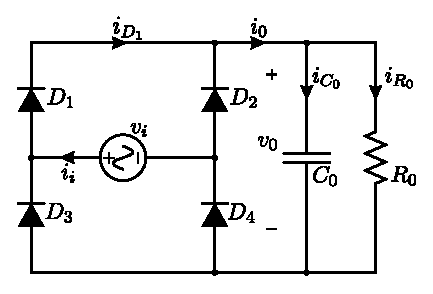
\includegraphics[width=0.65\linewidth]{Figs/RetOndaCompletaRC}
	\caption{Retificador de onda completa com filtro capacitivo.}
	\label{fig:retondacompletarc}
\end{figure}






\section{Estudo teórico}

Esta seção tem o objetivo de apresentar o embasamento teórico necessário para o entendimento da solução apresentada (ver Planilha). 
\begin{enumerate}	
	\item Apresente uma tabela com os valores dos componentes utilizados. (Tensão de entrada, frequência, resistência, capacitância...) 								
	\item  Apresente a expressão para o cálculo da ondulação da tensão de saída ($\Delta V_{C0}$) \eqref{eq:DeltaVC0}.
		\begin{equation}\label{eq:DeltaVC0}
		\Delta {V_{{C_0}}} = \frac{{\pi \hat V}}{{{\omega _0}{R_0}{C_0}}}
		\end{equation}
%onde: 
%
%\symboldescription{$\Delta {V_{{C_0}}}$}{ondulação de tensão no capacitor;}
%\symboldescription{$\omega _0$}{velocidade angular;}
%\symboldescription{$\hat V$}{tensão de pico de alimentação;}
%\symboldescription{$C_0$}{capacitância de carga;}
%\symboldescription{$R_0$}{resistência de carga;}
%	
	\item Apresente a expressão para o cálculo do valor médio da tensão de saída ($\bar{V_0}$) \eqref{eq:V0med}.
	
		\begin{equation}\label{eq:V0med}
	{\overline V _0} = \hat V - \frac{{\Delta {V_{{C_0}}}}}{2} = \hat V - \frac{{\pi \hat V}}{{2{\omega _0}{R_0}{C_0}}}
	\end{equation}
	
	\item  Apresente a expressão para o cálculo do ângulo de condução $\gamma_D$ do diodo $D_1$ \eqref{eq:AngCond} e do tempo de condução $t_D$ do mesmo \eqref{eq:TempoCond}.
	\begin{equation}\label{eq:AngCond}
	{\gamma _D} = \frac{1}{{\sqrt {{f_0}{R_0}{C_0}} }}
	\end{equation}
	
	\begin{equation}\label{eq:TempoCond}
	{t_D} = \frac{{{\gamma _D}}}{{{\omega _0}}} = \frac{1}{{{\omega _0}\sqrt {{f_0}{R_0}{C_0}} }}
	\end{equation}
		
%	\item  Apresente a expressão para o cálculo do valor de pico da corrente de carga ($\hat{I_0}$), valor médio ($\bar{I_0}$).
	\item Apresente a expressão para o fator de crista \eqref{eq:FatorCrista}, ou seja, a relação do valor de pico da corrente de entrada ($\hat{I_i}$) pelo valor eficaz (${I_i}$).
	\begin{equation}\label{eq:Iipico}
	{{\hat I}_i } = {\omega _0}{C_0}{{\hat V}_i}{\gamma _D} 
	\end{equation}
	
	\begin{equation}\label{eq:Iieficaz}
	{I_i} = {{\hat I}_i }\sqrt {\frac{{{\gamma _D}}}{{3\pi }}} 
	\end{equation}
	
	\begin{equation}\label{eq:FatorCrista}
	{F_C} = \frac{{{{\hat I}_i }}}{{{I_i}}} = \sqrt {\frac{{{\gamma _D}}}{{3\pi }}} 
	\end{equation}
	
	\item Apresente a expressão para o cálculo do fator de potência da estrutura.
	
\end{enumerate}


\section{Verificação por simulação}


A análise teórica apresentada anteriormente deve ser verificada por simulação.
\begin{enumerate}									
	\item   Apresente as formas de onda da tensão de saída em comparação com a tensão de saída sem o capacitor de filtro $|\sin(\omega_0 t)|$. Verifique o valor médio obtido por simulação com o teórico.
	\item   Apresente as formas de onda da corrente ($i_i$) de entrada e no diodo $D_1$. Verifique o cálculo do valor de pico e do valor médio.
	\item   Verifique o cálculo do tempo de condução do diodo.
	\item   Verifique o cálculo do fator de potência da estrutura.
	\item  Comente sobre as aproximações realizadas, dependendo dos parâmetros, por exemplo, sem a resistência de entrada (\emph{shunt}) a corrente de carga tem um formato triangular. Com a adição da resistência de entrada, a corrente passa a ter um formato senoidal.
\end{enumerate}





%Body Text
\section{Resultados experimentais}


A análise teórica, assim como as simulações, são verificadas de forma definitiva com os resultados experimentais.
\begin{enumerate}									
	\item   Descrever o experimento. Listar o material utilizado.  
	\item  Verificar experimentalmente cada item simulado na seção anterior;
	\item  Apresente uma fotografia do protótipo montado;
	\item  Salve as aquisições em formato .png e as coloque aqui, afim de verificar a operação adequada do retificador.
\end{enumerate}

A \tabref{tab:componentesRetificador} apresenta a lista de componentes utilizados...

\begin{table}[!ht]
	\centering
	\caption{Componentes utilizados na montagem do retificador}
	\label{tab:componentesRetificador}
	\begin{tabular}{@{}ccc@{}}
		\toprule
		\textbf{Componente} & \textbf{Descrição} & \textbf{Quantidade} \\ \midrule
		Resistores          & \SI{820}{\ohm} -- \SI{5}{\W}             & 4                   \\
		Resistor shunt      & \SI{0.1}{\ohm} -- \SI{5}{\W}             & 2                   \\
		Diodos              & 1N4007             & 4                   \\
		Capacitor           & \SI{220}{\micro\farad} x \SI{250}{\V}      & 1                   \\
		Conector Borne      &  KRE 2 Vias    & 2                   \\
		Fusível/Porta Fusível     &  \SI{5}{\A}  & 1                  \\
		Placa padrão        & \SI{10}{\cm} por \SI{10}{\cm}         & 1                   \\ \bottomrule
	\end{tabular}
\end{table}



\section{Conclusões} 

Por fim, apresenta-se uma conclusão sobre o trabalho estudado.
\begin{enumerate}								
	\item  Desfecho do trabalho. Problemas encontrados, soluções alcançadas...
	\item  Análise crítica, sugestões...
	%	\bonuspart[01] Parte extra.		
\end{enumerate}


As conclusões devem ser as mais claras possíveis, informando aos leitores sobre a importância do trabalho dentro do contexto em que se situa. As vantagens e desvantagens em relação aos já existentes na literatura devem ser comentadas, assim como os resultados obtidos e as possíveis aplicações práticas do trabalho.


\bibliographystyle{IEEEtran}

\bibliography{References} % Inclui arquivos de referência

\balance


